\documentclass[11pt]{article}
\usepackage[utf8]{inputenc}
\usepackage[T1]{fontenc}
\usepackage[main=czech]{babel}
\usepackage[nottoc]{tocbibind}
\usepackage{url}
\usepackage{xcolor}
\usepackage{minted}
\usepackage{array}
\usepackage{graphicx}
\usepackage{pgfplots}
\usepackage{wrapfig}

\usepackage{parskip}
\setlength{\parindent}{20pt}

\graphicspath{./images/}

\title{\textbf{FIT VUT Brno - IMS}\\
	2. Doprava zboží nebo osob\\
	Správa vícepatrového skladu}
\author{Daniel Dolejška, \texttt{xdolej08@stud.fit.vutbr.cz}}
\date{\today}

\begin{document}
	
	\maketitle
	\vfill
	\begin{figure}[hb]
		\centering
		
\includegraphics[width=0.65\textwidth]{images/fit-vutbr.png}
	\end{figure}
	
	\newpage
	\tableofcontents
	
	
	\newpage
	
	\section{Úvod}
	% Úvod musí vysvětlit, proč se celá práce dělá a
	%proč má uživatel výsledků váš dokument číst.
	%  Motivace a širší souvislosti. Kontext problému.
	%  V této práci je řešena implementace ..., která bude použita pro
	%sestavení modelu ...
	%  Na základě modelu a simulačních experimentů bude ukázáno
	%chování systému ... v podmínkách ...
	%  Smyslem experimentů je demonstrovat, že pokud by ..., pak by
	%...
	%  Správnost zvolené koncepce byla ověřena...
	% Psaní úvodů je náročná práce. Úvody se čtou!!!
	Tato práce se zaobírá modelováním\cite[str.~8]{ims-prezentace} vícepatrového skladu.
	Klíčovým prvkem tohoto systému\cite[str.~7]{ims-prezentace} je pohyb palet se zbožím mezi jednotlivými patry.
	
	Přesun palet mezi patry je možný pouze za pomoci vysokozdvižných vozíků.
	Pro účely přesunu palet mezi patry je vyhrazen jeden vysokozdvižný vozík.
	
	S vozíky mají z bezpečnostních důvodů oprávnění pracovat pouze určití zaměstnanci.
	Další podrobnosti systému viz Kapitola \ref{sec:rozbor}.
	
	Cílem této práce je zjistit následující:
	\begin{itemize}
		\item kolik času je ztraceno v průběhu přesunu palet mezi patry
		\item průměrné vytížení vozíku přesunem palet mezi patry
	\end{itemize}

	A na základě těchto informací dále zjistit k jaké úspoře by došlo v případě nahrazení vozíku výtahem a kolik by systém s výtahem dokázal efektivně "support" zaměstnanců.

	\subsection{Zdroje faktů}
	%1.1 Zdroje faktů
	% Kdo se na práci podílel jako autor, odborný
	%konzultant, dodavatel odborných faktů,
	%  význačné zdroje literatury/fakt, ...
	%  je ideální, pokud jste vaši koncepci konzultovali s nějakou
	%autoritou v oboru (v IMS projektu to je hodnoceno, ovšem
	%není vyžadováno)
	%  pokud nebudete mít odborného konzultanta, nevadí. Nelze
	%ovšem tvrdit, že jste celé dílo vymysleli s nulovou interakcí s
	%okolím a literaturou.
	% Zdroj údajů
	Fakta o tomto systému jsou původem z několika zdrojů - prvním je osobní zkušenost a pozorování.
	Mezi další zdroje informací a faktů pak patří zaměstnanci firmy, pracující přímo na skladě.


	\subsection{Ověření validity}
	%1.2 Ověření validity/funkčnosti
	% V jakém prostředí a za jakých podmínek
	%probíhalo experimentální ověřování validity
	%modelu.
	% Pokud čtenář/zadavatel vaší zprávy neuvěří ve
	%validitu vašeho modelu, obvykle vaši práci
	%odmítne už v tomto okamžiku.
	% Alternativně lze zmínit v závěru experimentů.

	\newpage
	\section{Rozbor tématu a použitých metod/technologií} \label{sec:rozbor}
	% Podstatná fakta o systému musí být zdůvodněna a
	%podepřena důvěryhodným zdrojem (vědecký článek,
	%kniha, osobní měření a zjišťování). Alespoň jeden (lépe 2)
	%zdroj.
	% Fakta:
	%  Kterékoliv číslo, fakt, stav, vztah.
	%  Za každým takovým údajem musí následovat odkaz na zdroj (1
	%důvěryhodný nebo několik jiných).
	%  Hypotézy/předpoklady (podklady).
	% SHO: proces příchodů požadavků/doby obsluhy,
	%struktura systému, ...

	%Věrohodnost faktů
	% Zdroj literatury — články, normy, tech.
	%dokumenty.
	% Osobní/zprostředkované pozorování v terénu
	%— má však svoje náležitosti (např. měření
	%stochastického jevu).
	% Hypotézy — založené na podobném systému.
	\footnotetext[1]{Zdroj: Osobní měření}
	\footnotetext[2]{Zdroj: Zaměstnanec firmy}
	\begin{enumerate}
		\item Sklad se nachází na třech podlažích\footnotemark[1]
		\begin{itemize}
			\item \textsf{Přízemí} - práce s vysokozdvižnými vozíky není nutná
			\item \textsf{1. a 2. podlaží} - paletu je nutné vždy dostat o patro níže
		\end{itemize}
		\item Ve skladě je jeden vozík vyhrazen pro přesun palet mezi patry\footnotemark[1]
		\begin{itemize}
			\item \textsf{20\%} ze zaměstnanců s vozíky pracovat nemůže a musí proto požádat jiného zaměstnance o pomoc, hledání trvá \textsf{30s - 2 minuty}\footnotemark[1]
		\end{itemize}
		\item Příchody zaměstnanců\footnotemark[2]
		\begin{itemize}
			\item \textsf{8} pracovníků přichází v 6 hodin
			\item \textsf{12} dalších pracovníků přichází v 9 hodin
		\end{itemize}
		\item Pracovní doba zaměstnanců\footnotemark[2]
		\begin{itemize}
			\item \textsf{8 hodin} pracovní doby
			\item Po \textsf{4 hodinách} si pracovníci berou \textsf{30 min} pauzu, přičemž rozpracované zakázky jsou vždy dokončeny
		\end{itemize}
		\item Za den je průměrně zpracováno (vyskladněno) 310 zakázek\footnotemark[2]
		\begin{itemize}
			\item \textsf{75\%} začíná ve 2. patře, následně pokračuje do prvního patra
			\item \textsf{20\%} začíná v 1. patře, následně pokračuje do přízemí
			\item \textsf{5\%} pouze z přízemí
		\end{itemize}
		Na základě poskytnutých statistických údajů\footnotemark[2] bylo zjištěno, že délka zpracování jedné zakázky se řídí normálním rozdělením\cite[str.~93]{ims-prezentace} se středem 30 minut a rozptylem 6 minut.\footnotemark[1]
		Tyto hodnoty byly upraveny na základě několika prvotních experimentů.
		
		Dále přiřazení nové zakázky (výběr, tisk, …) trvá průměrně 1 minutu.\footnotemark[1]
		
	\end{enumerate}
	
	\subsection{Použité postupy}
	Hlavním použitým postupem je vytvoření konceptuálního modelu\cite[str.~48]{ims-prezentace} pomocí P/T Petriho sítě\cite[str.~123]{ims-prezentace}.
	Ta byla využita především proto, že pomocí ní je vytvoření modelu systému hromadné obsluhy\cite[str.~136]{ims-prezentace} snadné a srozumitelné.
	
	Petriho síť v tomto případě popisuje především chování pracovníků v rámci skladu, jejich vstup do systému a dále i výstup.
	
	\subsection{Původ postupů}
	
	
	
	\section{Koncepce - modelářská témata}
	%3. Koncepce modelu/simulátoru
	%  Konceptuální model je abstrakce reality a redukce reality
	%na soubor relevantních faktů pro sestavení simulačního
	%modelu.
	% Pokud některé partie reality zanedbáváte nebo
	%zjednodušujete, musí to být zdůvodněno a v
	%ideálním případě musí být prokázáno, že to
	%neovlivní validitu modelu.
	% Výsledek kapitoly: konceptuální (abstraktní)
	%model s vyznačením relevantních faktů.
	% Základní koncept modelu.
	
	%Fakta versus Koncepce
	% Fakta: soupis znalostí o daném problému.
	% Koncepce:
	%  převzetí faktů do modelu,
	%  zdůvodněné provedené zjednodušení faktů,
	%  abstraktní popis modelu/programu.
	% Těžiště modelářské práce. Vytváříme abstraktní
	%model.
	% Návod: koncepci vaší práce MUSÍ pochopit
	%libovolný technik (a často i manažer...).
	
	%Koncepce SHO: Petriho síť
	% Může být dobré ukázat vztahy mezi procesy a
	%zdroji v systému.
	%  Neberme AM v Petriho síti jako detailní program.
	%AM má ukázat zásadní fakta o systému. Části, které v PS
	%nelze vyjádřit, vyjádřete slovním popisem.
	%  Konkrétní fronta se volí podle.... Vygeneruje se normal(X,Y)
	%značek...
	% AM musí být stručný, přehledný a srozumitelný
	%Může být čitelně psán rukou + scan.
	
	%Zjišťování faktů
	% Náročná práce, mnohdy téměř partyzánská.
	% Literatura.
	% Osobní (nedestruktivní) zjišťování v terénu.
	% Je to součást modelářské práce.
	
	Některé vlastnosti reálného systému jsou pro účely vytvoření simulačního modelu zanedbány, např.:
	\begin{itemize}
		\item Pozdní, či brzké příchody pracovníků jsou zcela zanedbávány, simulační model vždy pracuje s včasným příchodem zaměstnanců.
		Pokud se odchylky drží v určitých mezích (+/-5 minut) nehrají v simulačním modelu téměř žádnou roli.
	\end{itemize}
	
	\subsection{Popis konceptuálního modelu}
	Model je popsán dvěma vizuálně oddělenými Petriho sítěmi, které dohromady tvoří jedinou síť.
	Obě sítě obsahují stav \textsf{PR-V} - ten reprezentuje jeden jediný stav, který spojuje obě sítě.
	
	\subsubsection{Chod skladu}
	Chod skladu je znázorněn na obrázku \ref{obr:petriho-sit-sklad} (strana \pageref{obr:petriho-sit-sklad}).
	
	Ze stavu, kdy pracovník vstoupil do systému, vrátil se z pauzy či dokončil zakázku (\texttt{PR-V}) po 1 minutu přijímá zakázku novou (\texttt{ZAK}).
	Po přijetí nové zakázky existuje 75\% pravděpodobnost, že se objednávka musí začít připravovat v druhém patře (\texttt{ZAK-P2}), 20\% v prvním patře (\texttt{ZAK-P1}) a 5\% v přízemí (\texttt{ZAK-P0}).
	Následně se objednávka v daných patrech po danou dobu zpracovává (\texttt{PRAC-P2/P1/P0}).
	Doba zpracování je určena normálním rozdělením se středem 30 minut a rozptylem 6 minut.
	Model předpokládá, že pracovník na všech patrech pracuje stejně dlouhou dobu (třetinu z celkového času zpracování objednávky).
	
	Po dokončení zpracování zakázky v prvním či druhém patře (\texttt{PR-P2/P1-H}) existuje 20\% šance (\texttt{P2/P1-VO-N}), že daný pracovník nemůže operovat s vysokozdvižným vozíkem a musí proto požádat jiného zaměstnance o pomoc při přesunu palety o patro níže.
	Hledání odpovídajícího pracovníka trvá 30 sekund až 2 minuty (\texttt{P2/P1-VO-H}).
	
	Pro přesun palet mezi patry a do přízemí je vyhrazen jeden vozík (\texttt{VOZIK}).
	Samotný přesun palety trvá 30 sekund až minutu (\texttt{P2/P1-VO-U}).
	Po přesunutí palety do nižšího patra probíhá práce na daném patře a celý proces přesunu palety se opakuje, dokud paleta nedorazí do přízemí (\texttt{PR-P0}).
	
	V přízemí se po dokončení práce (\texttt{PRAC-P0}) paleta zanechá na určeném místě a pracovník se vrací do výchozího stavu (\texttt{PR-V}).
	
	\subsubsection{Vstupy a výstupy pracovníků skladu}
	Vstupy a výstupy procesů jsou znázorněny na obrázku \ref{obr:petriho-sit-vstupvystup} (strana \pageref{obr:petriho-sit-vstupvystup}).
	
	Bezprostředně na začátku do systému vstupuje 8 pracovníků (\texttt{PR-P}). Po 3 hodinách (\texttt{PRCH-DOP}) do skladu vstupuje 12 dalších pracovníků (\texttt{DOP}).
	
	Každý z nich ve skladě pracuje 8 hodin (\texttt{PRACE}, 30 min kompenzuje délku přestávky).
	Po čtyřech hodinách (\texttt{PRES-PRAC}) práce pracovník odchází (\texttt{PRES-VS}) na třicetiminutovou přestávku (\texttt{PRES}) (jakékoli rozpracované zakázky nejdříve dokončí), poté se do systému vrací a pokračuje v práci (\texttt{PR-V}).
	
	\subsection{Konceptuální model}
	\begin{figure}[h!]
		\caption{Petriho síť popisující chod skladu}
		\centering
		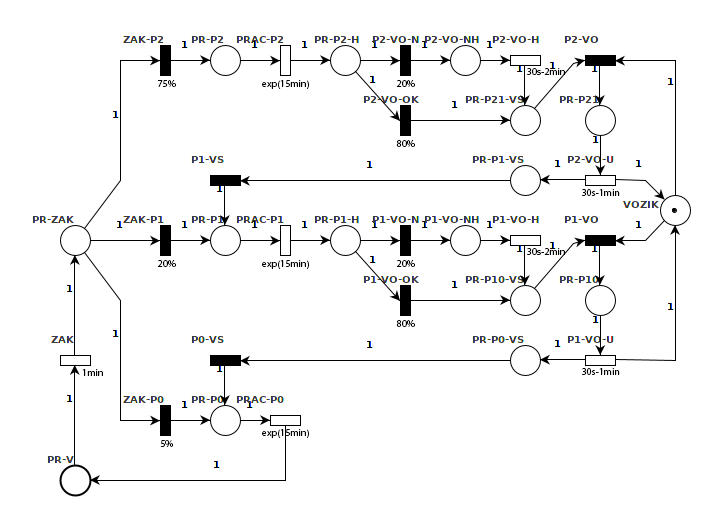
\includegraphics[width=\textwidth]{images/petri_net_sklad.png}
		\label{obr:petriho-sit-sklad}
	\end{figure}

	\begin{figure}[h!]
		\caption{Petriho síť popisující vstup a výstup pracovníků do/ze systému}
		\centering
		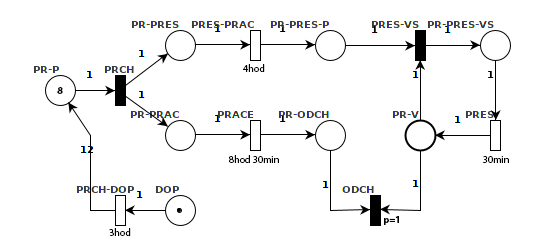
\includegraphics[width=\textwidth]{images/petri_net_prichody.png}
		\label{obr:petriho-sit-vstupvystup}
	\end{figure}
	
	
%	\section{Koncepce - implementační témata}
%	Simulační model využívá především funkcionalitu pro diskrétní simulace[str 119] z knihovny SIMLIB[XXXXXX].
%	
%	Podle specifikace konceptuálního modelu se v simulačním modelu pohybují procesy[str 121] (které v tomto případě reprezentují především pracovníky skladu) v různých stavech, zabírají obslužné linky[str 146] a simulují činnost.
%	Objekty sbírají v průběhu simulace důležité statistické informace, ze kterých je možné zjistit klíčové vlastnosti modelovaného systému.
	
	\newpage
	\section{Architektura simulačního modelu/simulátoru}
	Simulační model využívá především funkcionalitu pro diskrétní simulace[str 119] z knihovny SIMLIB\cite{simlib}.
	
	Podle specifikace konceptuálního modelu se v simulačním modelu pohybují procesy[str 121] (které v tomto případě reprezentují především pracovníky skladu) v různých stavech, zabírají obslužné linky[str 146] a simulují činnost.
	Objekty sbírají v průběhu simulace důležité statistické informace, ze kterých je možné zjistit klíčové vlastnosti modelovaného systému.
	
	\subsection{Mapování abstraktního modelu}
	XXXXXXXXXXXXXXXXXXXXXXX
	
	
	\section{Podstata simulačních experimentů a jejich průběh}
	%Simulační studie začíná formulováním problému:
	%  co chci zjistit,
	%  (proč je k tomu potřeba simulační model.)
	% Studie končí výslovením závěru:
	%  co jsem tedy zjistil,
	%  co bych ještě mohl zjistit,
	%  (proč by to nešlo bez modelu.)
	%  Bez experimentů práce nedává smysl!
	Cílem této studie je pomocí experimentů zjistit jaké je vytížení vysokozdvižného vozíku pro přesun palet mezi patry a jaký to má dopad na zpracování zakázek.
	
	Dále také porovnat existující systém s modelem, ve kterém byl vysokozdvižný vozík nahrazen výtahem spojující všechna patra skladu.
	
	\subsection{Postup experimentování}
	Prvotní experimenty se simulačním modelem byly nejprve cíleny na ověření správné činnosti modelu (kontrola správných počtů přestávek, pracovní doby a rychlosti zpracovávání zakázek) a na základě výsledků byly opraveny chyby, které byly experimenty odhaleny.
	
	Nejprve je zkoumáno chování modelu s výchozími parametry dle specifikací systému. Následně se zkoumá, jak se systém chová pří zvýšení či snížení těchto hodnot. V poslední řadě se zjišťuje chování systému s extrémními hodnotami (v rámci validity modelu).
	
	\subsection{Jednotlivé experimenty}
	Pokud není v uvedeno jinak byly tyto simulační experimenty prováděny s výchozím počtem pracovníků skladu a jediným vysokozdvižným vozíkem (dle specifikovaných fakt o systému). Simulován byl dlouhodobý provoz skladu - přesněji 261 dní (počet pracovních dní v roce).
	
	\subsubsection{Vytížení vozíku a jeho dopad na práci}
	Na základě simulačních experimentů bylo zjištěno, že samotný vysokozdvižný vozík zpožďuje každým přesunem každou zakázku o průměrně 1 minutu a v rušných chvílích až o 7 minut.
	
	Celý proces přesunu palet v rámci všech pater zpožďuje zakázky v průměru o téměř 3 minuty a v extrémních případech až o 10-13 minut. Tento proces zahrnuje hledání pracovníků pro přesun palety, čekání ve frontě i samotný přesun.
	
	\begin{tikzpicture}
	\label{graf:zpozdeni-standard}
	\begin{axis}[
	ybar,
	title={Graf 1: Maximální celkové zpoždění zakázky přesuny palet},
	title style={yshift=1.5ex},
	xtick=data,
	xlabel={Maximální zpoždění [min]},
	ylabel={Počet zakázek [desetitisíce]},
	x=0.74cm,
	nodes near coords, 
	nodes near coords align={vertical},
	point meta=y,
	enlargelimits=0.15,
	bar width=9pt,
	xmajorgrids=false,
	ymajorgrids=true,
	grid style=dashed,
	]
	\addplot
	coordinates {(1,10443)(2,18498)(3,20043)(4,15974)(5,9626)(6,5098)(7,2272)(8,853)(9,305)(10,90)(11,29)(12,6)(13,1)};
	\end{axis}
	\end{tikzpicture}
	
	\subsubsection{Nahrazení vozíku výtahem}
	Výtah v simulačním modelu má následující parametry:
	\begin{itemize}
		\item výtah se přesune z jednoho patra do druhého za 8 vteřin
		\item do výtahu se vejde pouze jedna paleta a smí jej použít kdokoliv
	\end{itemize}

	V modelu, kde byl vozík nahrazen výtahem bylo zpoždění zakázek přesunem palety mezi patry značně sníženo.
	Průměrné zpoždění zakázky přesunem nedosahuje ani 15 vteřin, s maximálním zpožděním 1 minutu a 40 vteřin.

	\begin{wrapfigure}{r}{0.5\textwidth}
		\begin{tikzpicture}
			\label{graf:zpozdeni-vytah}
			\begin{axis}[
				ybar,
				title={Graf 2: Maximální celkové zpoždění zakázky\\přesuny palet,
					model s výtahem},
				title style={align=center,yshift=1.5ex},
				x tick label style={
					/pgf/number format/1000 sep=},
				xlabel={Maximální zpoždění [min]},
				ylabel={Počet zakázek [desetitisíce]},
				x=1cm,
				y=1cm/50000,
				nodes near coords, 
				nodes near coords align={vertical},
				point meta=y,
				enlarge y limits=0.35,
				enlarge x limits=0.15,
				bar width=9pt,
				xmajorgrids=false,
				ymajorgrids=true,
				grid style=dashed,
			]
			\addplot 
				coordinates {(1,78539)(2,10604)(3,76)(4,1)(5,0)};
			\end{axis}
		\end{tikzpicture}
	\end{wrapfigure}
	
	Celý proces přesunu v rámci všech pater byl snížen na průměrně 40 vteřin, s maximálním registrovaným zpožděním 3-4 minut.
	Viz Graf 2 na straně \pageref{graf:zpozdeni-vytah}.
	
	Efektivně to vede ke snížení času nutného ke zpracování každé zakázky a k celkovému zvýšení efektivity modelovaného systému.
	Model vykazuje zvýšení zpracovaných zakázek o více než 7\%.
	
	Na Grafu 3 na straně \ref{graf:casy-zakazek-porovnani} lze pro výsledky modelu "Výtah" pozorovat vyšší počty zakázek s nižším časem pro jejich zpracování než pro výsledky modelu "Vozík".
	
	\begin{center}
	\begin{tikzpicture}
	\label{graf:casy-zakazek-porovnani}
	\begin{axis}[
	title={Graf 3: Porovnání časů zpracování zakázek},
	title style={align=center,yshift=1.5ex},
	x tick label style={
		/pgf/number format/1000 sep=},
	xlabel={Celkový čas zpracování zakázky [min]},
	ylabel={Počet zakázek [desetitisíce]},
	y=1cm/4000,
	x=1cm/7,
	point meta=y,
	enlargelimits=0.15,
	bar width=9pt,
	xmajorgrids=true,
	ymajorgrids=true,
	grid style=dashed,
	]
	\addplot 
	coordinates {(5,24)(10,2176)(15,2985)(20,5849)(25,12086)(30,16140)(35,19684)(40,15527)(45,6950)(50,1614)(55,196)(60,7)};
	\addplot 
	coordinates {(5,30)(10,2265)(15,4145)(20,9021)(25,16245)(30,20552)(35,20614)(40,12197)(45,3560)(50,557)(55,33)(60,1)};
	\legend{Vozík,Výtah}
	\end{axis}
	\end{tikzpicture}
	\end{center}
	
	\subsection{Závěry experimentů}
	Experimenty prokázaly...
	
	%Experimenty: úvod
	% Experimentování musí mít předem zvolený a zdůvodněný
	%řád, či postup.
	% Okolnosti experimentování:
	%  datová sada, konfigurace měřící aparatury, …
	%  závislost Y na X (graf).
	% Test versus Experiment.
	%  “měření” != experiment !!!
	% Experimenty se i ladí model - kalibrační experimenty.
	%  ... na základě tohoto experimentu jsme korigovali parametr x..
	%  u praktických simulačních studií se nepublikuje.
	%Struktura kapitoly Experimenty
	% 5.1 Postup experimentování a okolnosti studie
	% 5.2 Dokumentace jednotlivých experimentů
	% 5.3 Závěr experimentů
	% Poznámka: experimentování je činnost
	%vyžadující preciznost.
	%  modelování a SIMULACE
	%Dokumentace experimentu
	% Protokolární forma:
	%  vstupy a okolnosti,
	%  výstupy a pozorování,
	%  interpretace výsledků.
	% Interpretace výsledků:
	%  Rozbor výsledků: co v nich má čtenář vidět.
	%  Grafy mají pojmenované a kalibrované osy.
	% Návrh dalšího experimentu.
	%Závěry experimentů
	% Co bylo experimentováním zjištěno.
	% Jaké chyby v modelu byly odstraněny (oproti
	%původním předpokladům ... došlo ke změně
	%koncepce ... protože ...).
	% Co lze zjistit dalšími experimenty.
	
	
	\section{Shrnutí simulačních experimentů a závěr}
	%Jednoznačná odpověď na prvotní otázku studie.
	%  Studií provedenou na našem modelu bylo jednoznačně
	%prokázáno/vyvráceno, že ...
	%  V rámci experimentů bylo zjištěno, že průměrné zatížení ...
	%je ...
	%  Z experimentů vyplývá jednoznačné doporučení, aby
	%provozovatel ... rozšířil výrobu o ...
	%  Ze statisticky zpracovaného měření v terénu plyne, že proces
	%příchodů ... se řídí normálním rozložením se středem a ....
	%  Na přiložených demo-příkladech jsme ověřili funkčnost ...
	
	
	\newpage
	\bibliographystyle{plain}
	\bibliography{zdroje}
	
\end{document}
